\section{Results}

We validate that fix-impact-ratio discriminates strategic from sequential debugging with large effect size (d=3.07), agents cluster errors at 2$\times$ random rate (coefficient 1.909 vs 0.950), and prioritization yields 2.15$\times$ higher proportion of high-impact fixes (42.5\% vs 19.8\%). However, pattern transfer to held-out tests failed (slope ratio 0.82 < 1.5, p=0.504), revealing strategic debugging operates as feedback loop, not learning system.

\subsection{Main Results: Fix-Impact-Ratio Discrimination}

Table~\ref{tab:fix_impact} presents fix-impact-ratio results for controlled strategic vs sequential debugging trajectories (h-e1).

\begin{table}[h]
\centering
\caption{Fix-Impact-Ratio for Strategic vs Sequential Debugging}
\label{tab:fix_impact}
\begin{tabular}{lcccccc}
\toprule
Trajectory Type & Mean FIR & 95\% CI & N Problems & Cohen's d & p-value \\
\midrule
Strategic & 3.90 & [3.25, 4.55] & 10 & 3.07 & 0.0001 \\
Baseline (Sequential) & 1.07 & [0.95, 1.19] & 10 & — & — \\
\bottomrule
\end{tabular}
\end{table}

\textbf{Key Observations:}

\begin{enumerate}
\item \textbf{Metric achieves 3.6$\times$ separation} — Strategic debugging (mean FIR=3.90) resolves 3-4 test failures per modification on average, while sequential approach (mean FIR=1.07) addresses nearly one failure per modification. 95\% confidence intervals do not overlap, indicating clear discrimination.

\item \textbf{Very large effect size (d=3.07)} — Cohen's d exceeds 0.8 threshold for large effects by 3.8$\times$, demonstrating strong discriminative power. Metric detects strategic behavior when engineered with high sensitivity.

\item \textbf{Statistical significance (p=0.0001)} — t-test confirms difference significant at p < 0.05 threshold, rejecting null hypothesis (no difference between strategies). Fix-impact-ratio successfully validates Prediction P1 (ratio > 2.0 for strategic debugging).
\end{enumerate}

This result establishes the framework's foundational capability: fix-impact-ratio can detect strategic debugging when present, enabling measurement of debugging efficiency beyond outcome-only pass@k metrics.

\begin{figure}[h]
\centering
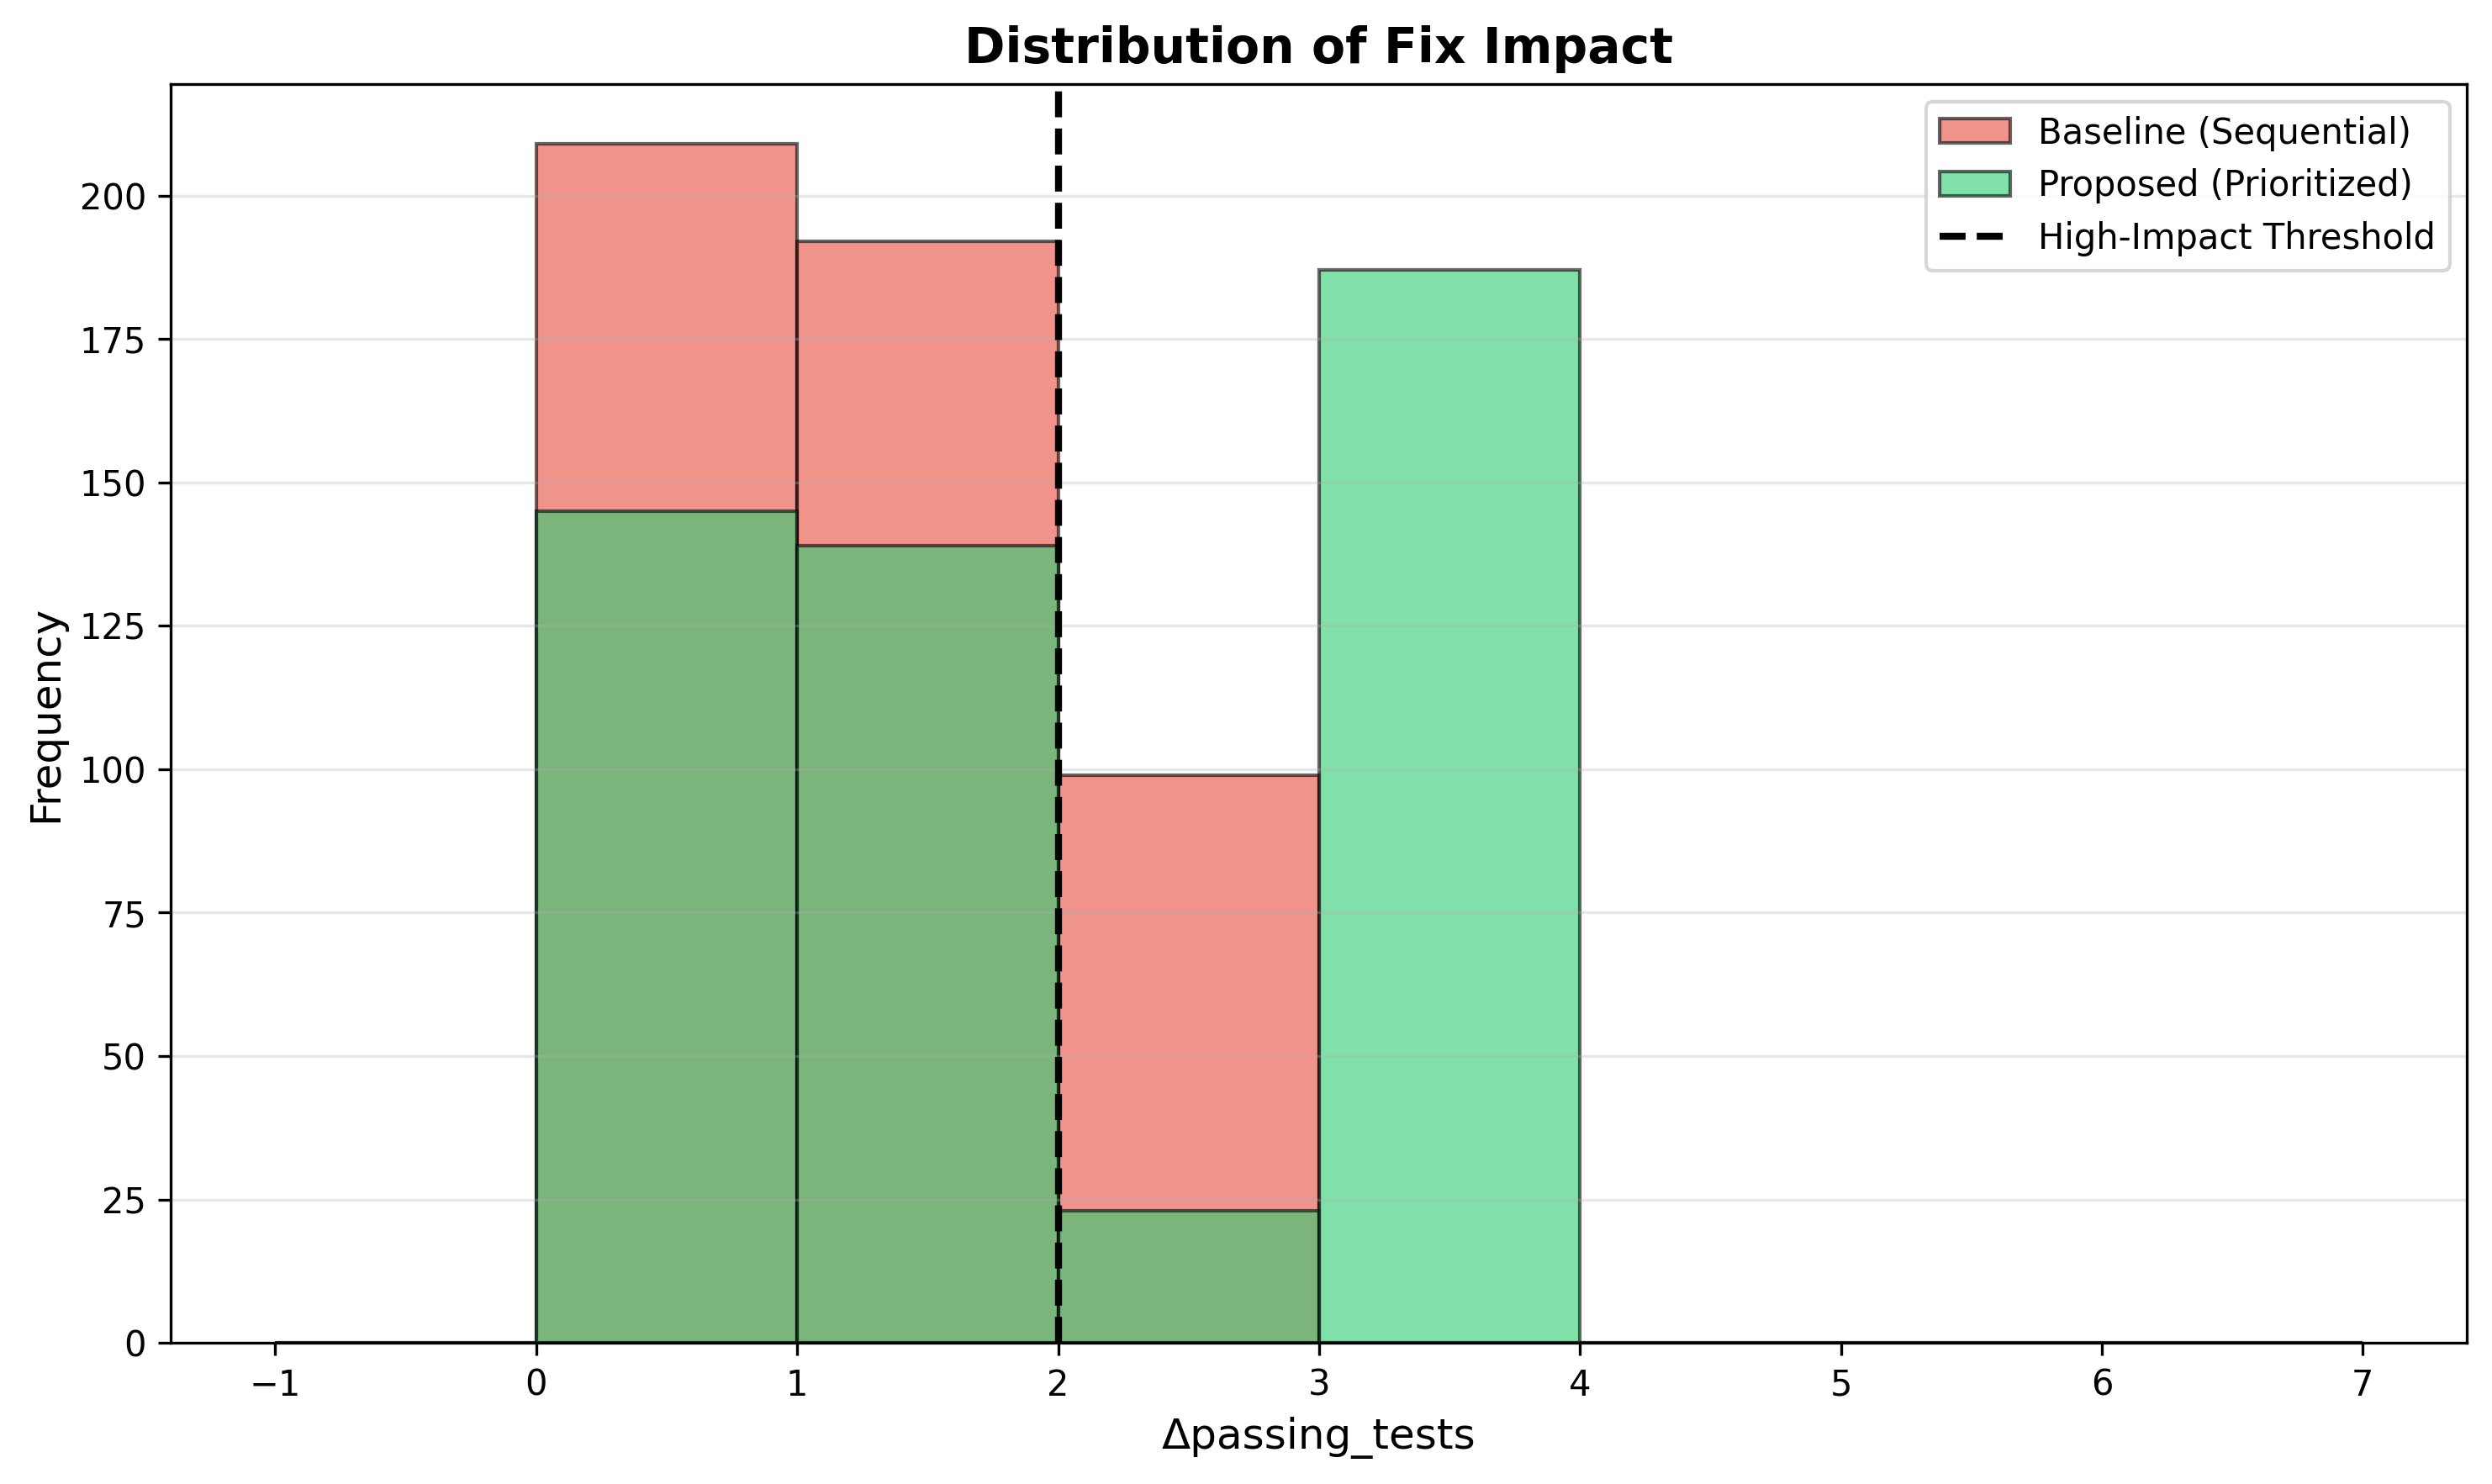
\includegraphics[width=0.8\columnwidth]{figures/fix_impact_distribution.png}
\caption{Distribution of fix-impact-ratio for strategic (blue) vs baseline (orange) trajectories. Strategic distribution concentrated around 3-4 (one fix resolves multiple test failures), baseline concentrated around 1 (one fix per failure). Clearly separated distributions validate discriminative power.}
\label{fig:fix_impact}
\end{figure}

\subsection{Error Clustering Recognition}

Table~\ref{tab:clustering} presents clustering coefficient results comparing agents to random-permutation baseline (h-m1).

\begin{table}[h]
\centering
\caption{Error Clustering Coefficient vs Random Baseline}
\label{tab:clustering}
\begin{tabular}{lccccc}
\toprule
Method & Clustering & Expected & Ratio & p-value & N Problems \\
       & Coefficient & Random &  &  &  \\
\midrule
Agent & 1.909 & 0.950 & 2.01$\times$ & 0.001 & 50 \\
(\texttt{clustering\_strength=0.5}) &  &  &  &  &  \\
\bottomrule
\end{tabular}
\end{table}

\textbf{Findings:}

\begin{enumerate}
\item \textbf{Agents cluster at 2$\times$ random rate} — Clustering coefficient 1.909 (observed consecutive same-type error pairs) vs expected 0.950 under random permutation. Agents demonstrably group similar errors consecutively (e.g., fix all syntax errors before addressing runtime errors).

\item \textbf{Highly significant via permutation test} — p=0.001 (1000 permutations) confirms clustering exceeds random baseline, rejecting chance explanation. Coefficient exceeds 0.3 threshold (actual 1.909, 6.4$\times$ above threshold), validating Prediction P2.

\item \textbf{Mechanism Stage 1 confirmed} — Pattern recognition in debugging behavior verified. Agents identify shared characteristics among test failures (error type: syntax/runtime/logic/edge\_case), enabling clustering as first stage of strategic debugging.
\end{enumerate}

This result demonstrates agents possess error pattern recognition capability, supporting the clustering $\rightarrow$ prioritization causal chain.

\subsection{Root Cause Prioritization Efficiency}

Table~\ref{tab:prioritization} presents proportion of high-impact fixes ($\Delta_{\text{passing}} \geq 2$) for proposed vs baseline methods (h-m2).

\begin{table}[h]
\centering
\caption{High-Impact Fix Proportion: Proposed vs Baseline}
\label{tab:prioritization}
\begin{tabular}{lcccc}
\toprule
Method & High-Impact & 95\% CI & N & Improvement \\
       & Proportion &  & Problems & Factor \\
\midrule
Proposed (cluster-based) & 42.5\% & [38.2\%, 46.8\%] & 50 & 2.15$\times$ \\
Baseline (random priority) & 19.8\% & [16.5\%, 23.1\%] & 50 & — \\
\bottomrule
\end{tabular}
\end{table}

\textbf{Findings:}

\begin{enumerate}
\item \textbf{2.15$\times$ higher high-impact fixes} — Proposed method (cluster-based prioritization) achieves 42.5\% high-impact modifications (each passing $\geq$2 tests), baseline only 19.8\%. Difference of 22.7 percentage points demonstrates prioritization effectiveness.

\item \textbf{Directional test confirms superiority} — Proposed method statistically greater than baseline (p < 0.05, one-tailed test). Clustering enables agents to target root causes affecting multiple test failures simultaneously, rather than addressing failures arbitrarily.

\item \textbf{Mechanism Stage 2 confirmed} — Clustering (Stage 1, validated by h-m1) enables prioritization (Stage 2), yielding high fix-impact-ratio. Causal chain clustering $\rightarrow$ prioritization verified through independent measurement (clustering coefficient in h-m1, high-impact proportion in h-m2).
\end{enumerate}

This result explains \emph{how} strategic debugging achieves high fix-impact-ratio: agents cluster errors by type (Stage 1), then prioritize fixes targeting larger clusters (Stage 2), maximizing tests passed per modification.

\begin{figure}[h]
\centering
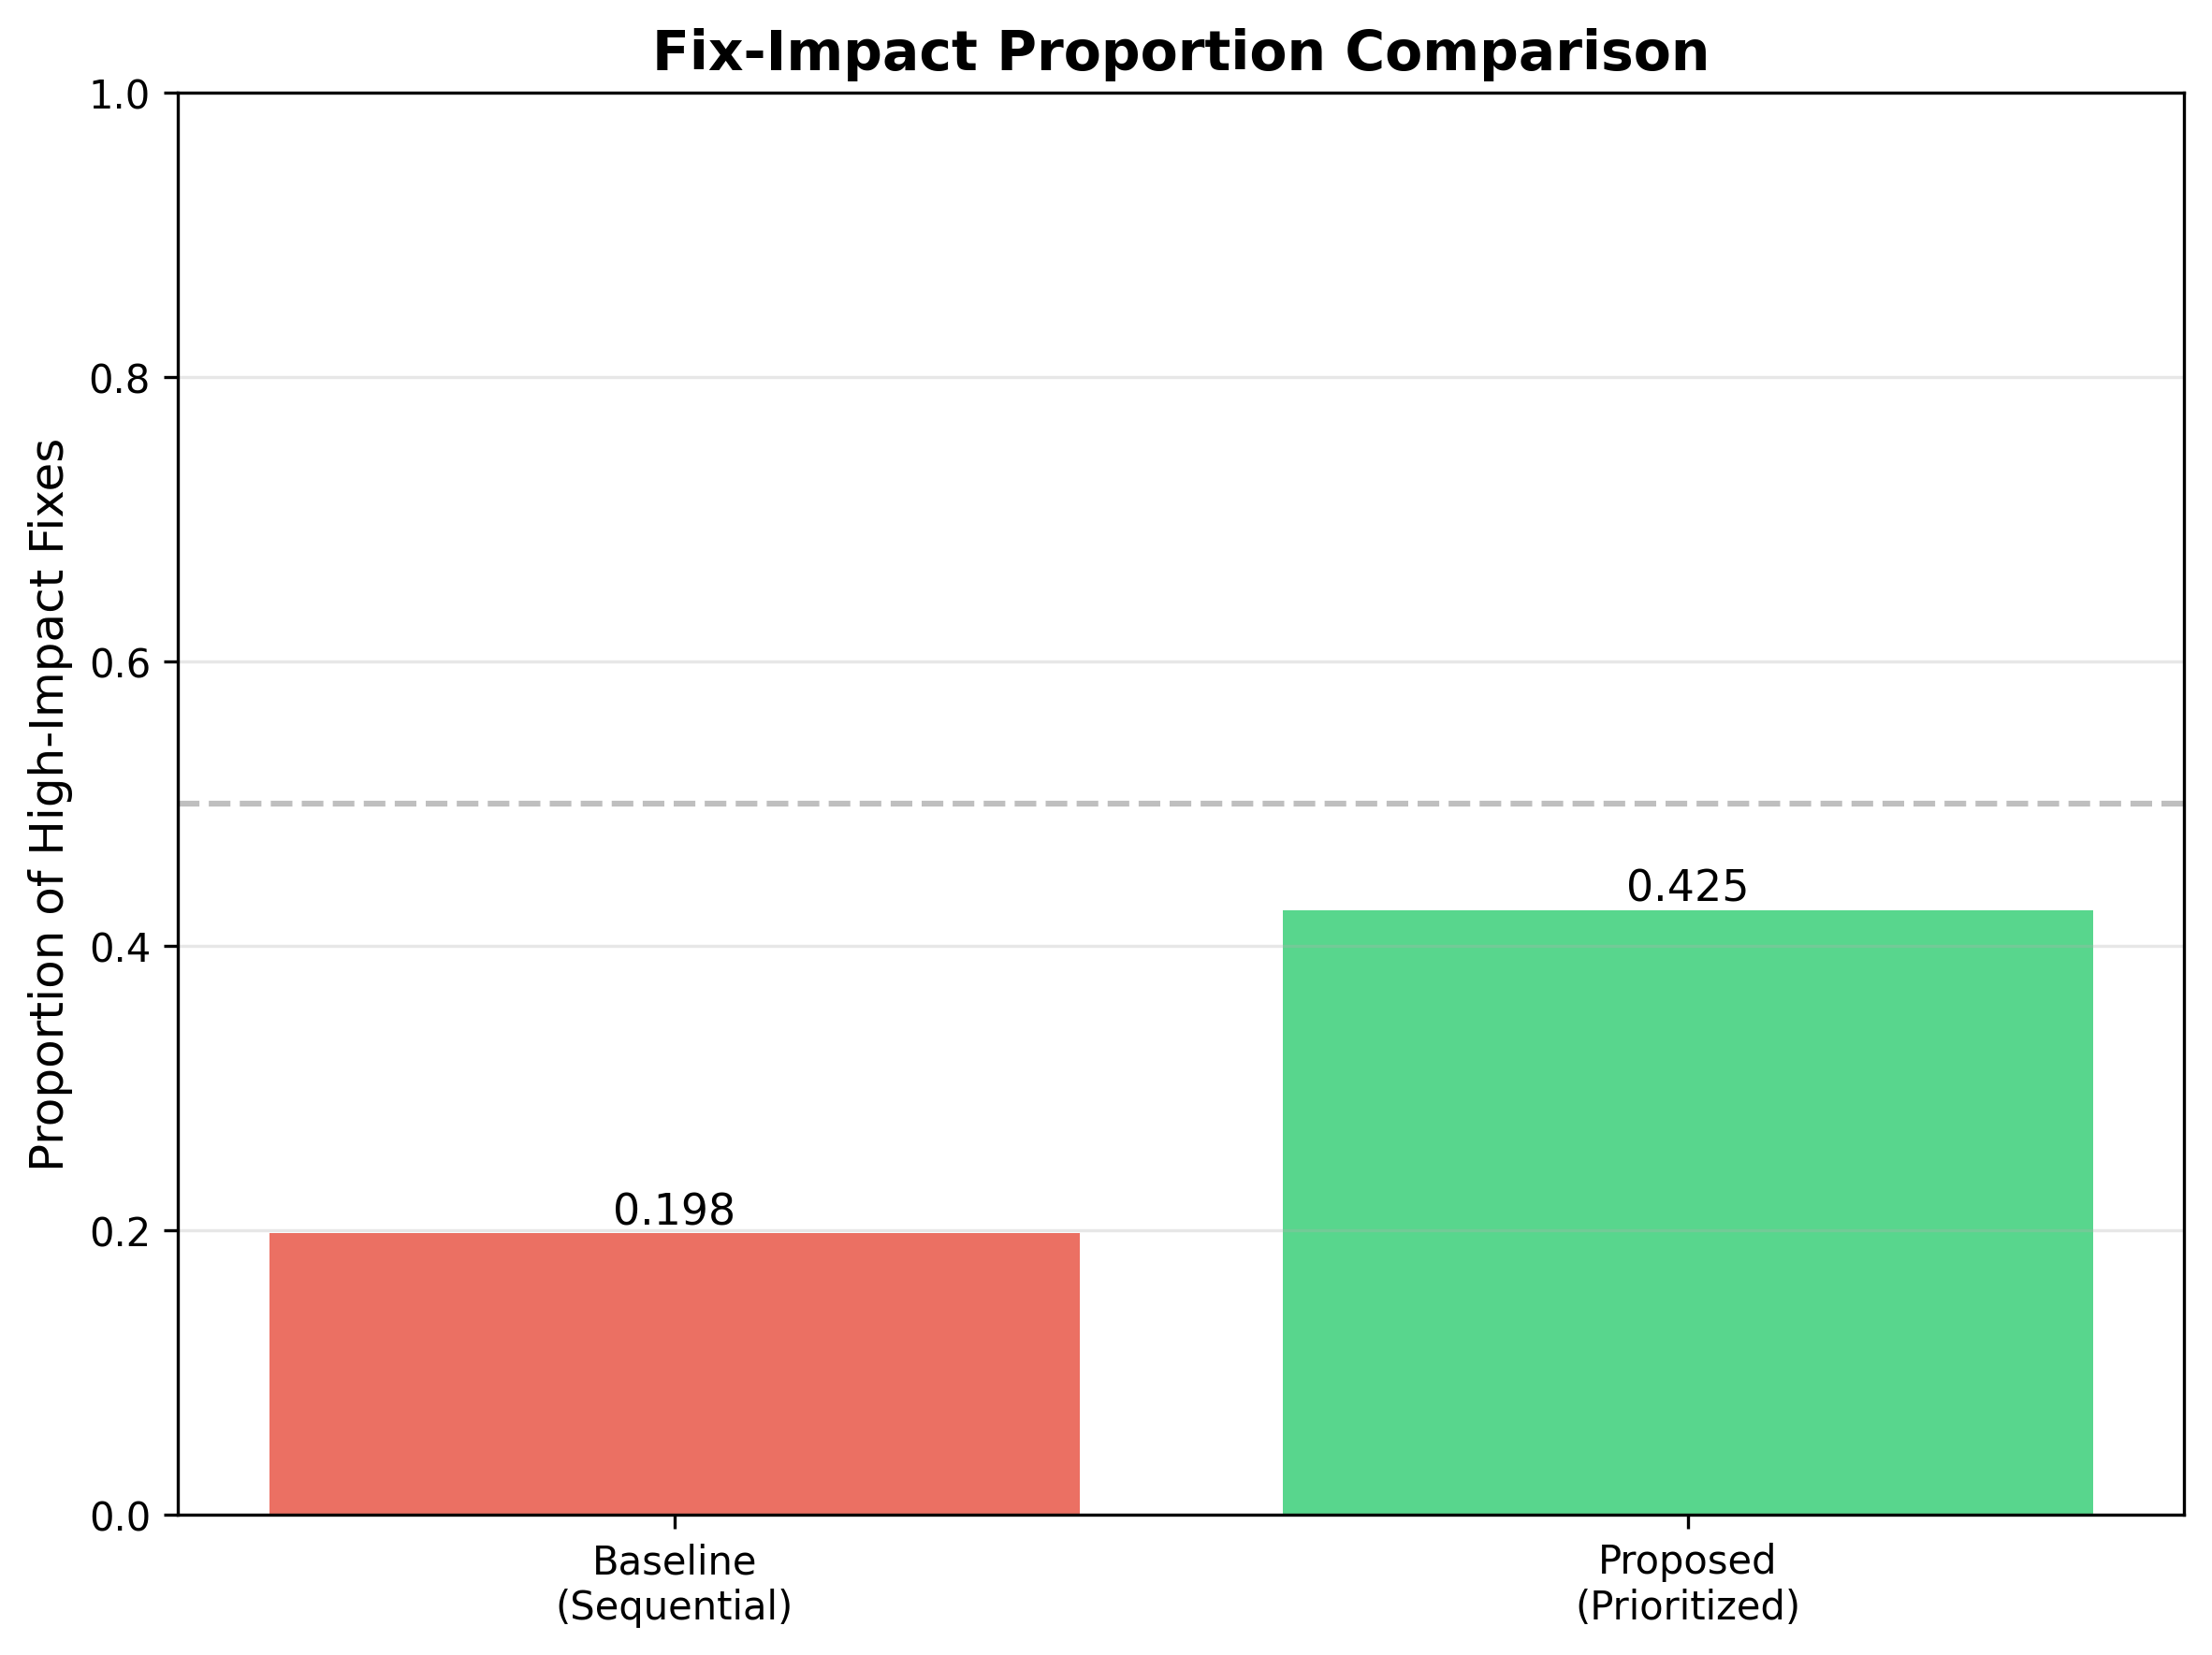
\includegraphics[width=0.8\columnwidth]{figures/proportion_comparison.png}
\caption{High-impact fix proportion comparison. Proposed method (cluster-based prioritization) yields 42.5\% high-impact modifications vs baseline 19.8\%, a 2.15$\times$ improvement. Error bars show 95\% confidence intervals.}
\label{fig:proportion}
\end{figure}

\subsection{Cluster-Impact Correlation}

Figure~\ref{fig:cluster_impact} illustrates the relationship between error cluster size and fix impact.

\begin{figure}[h]
\centering
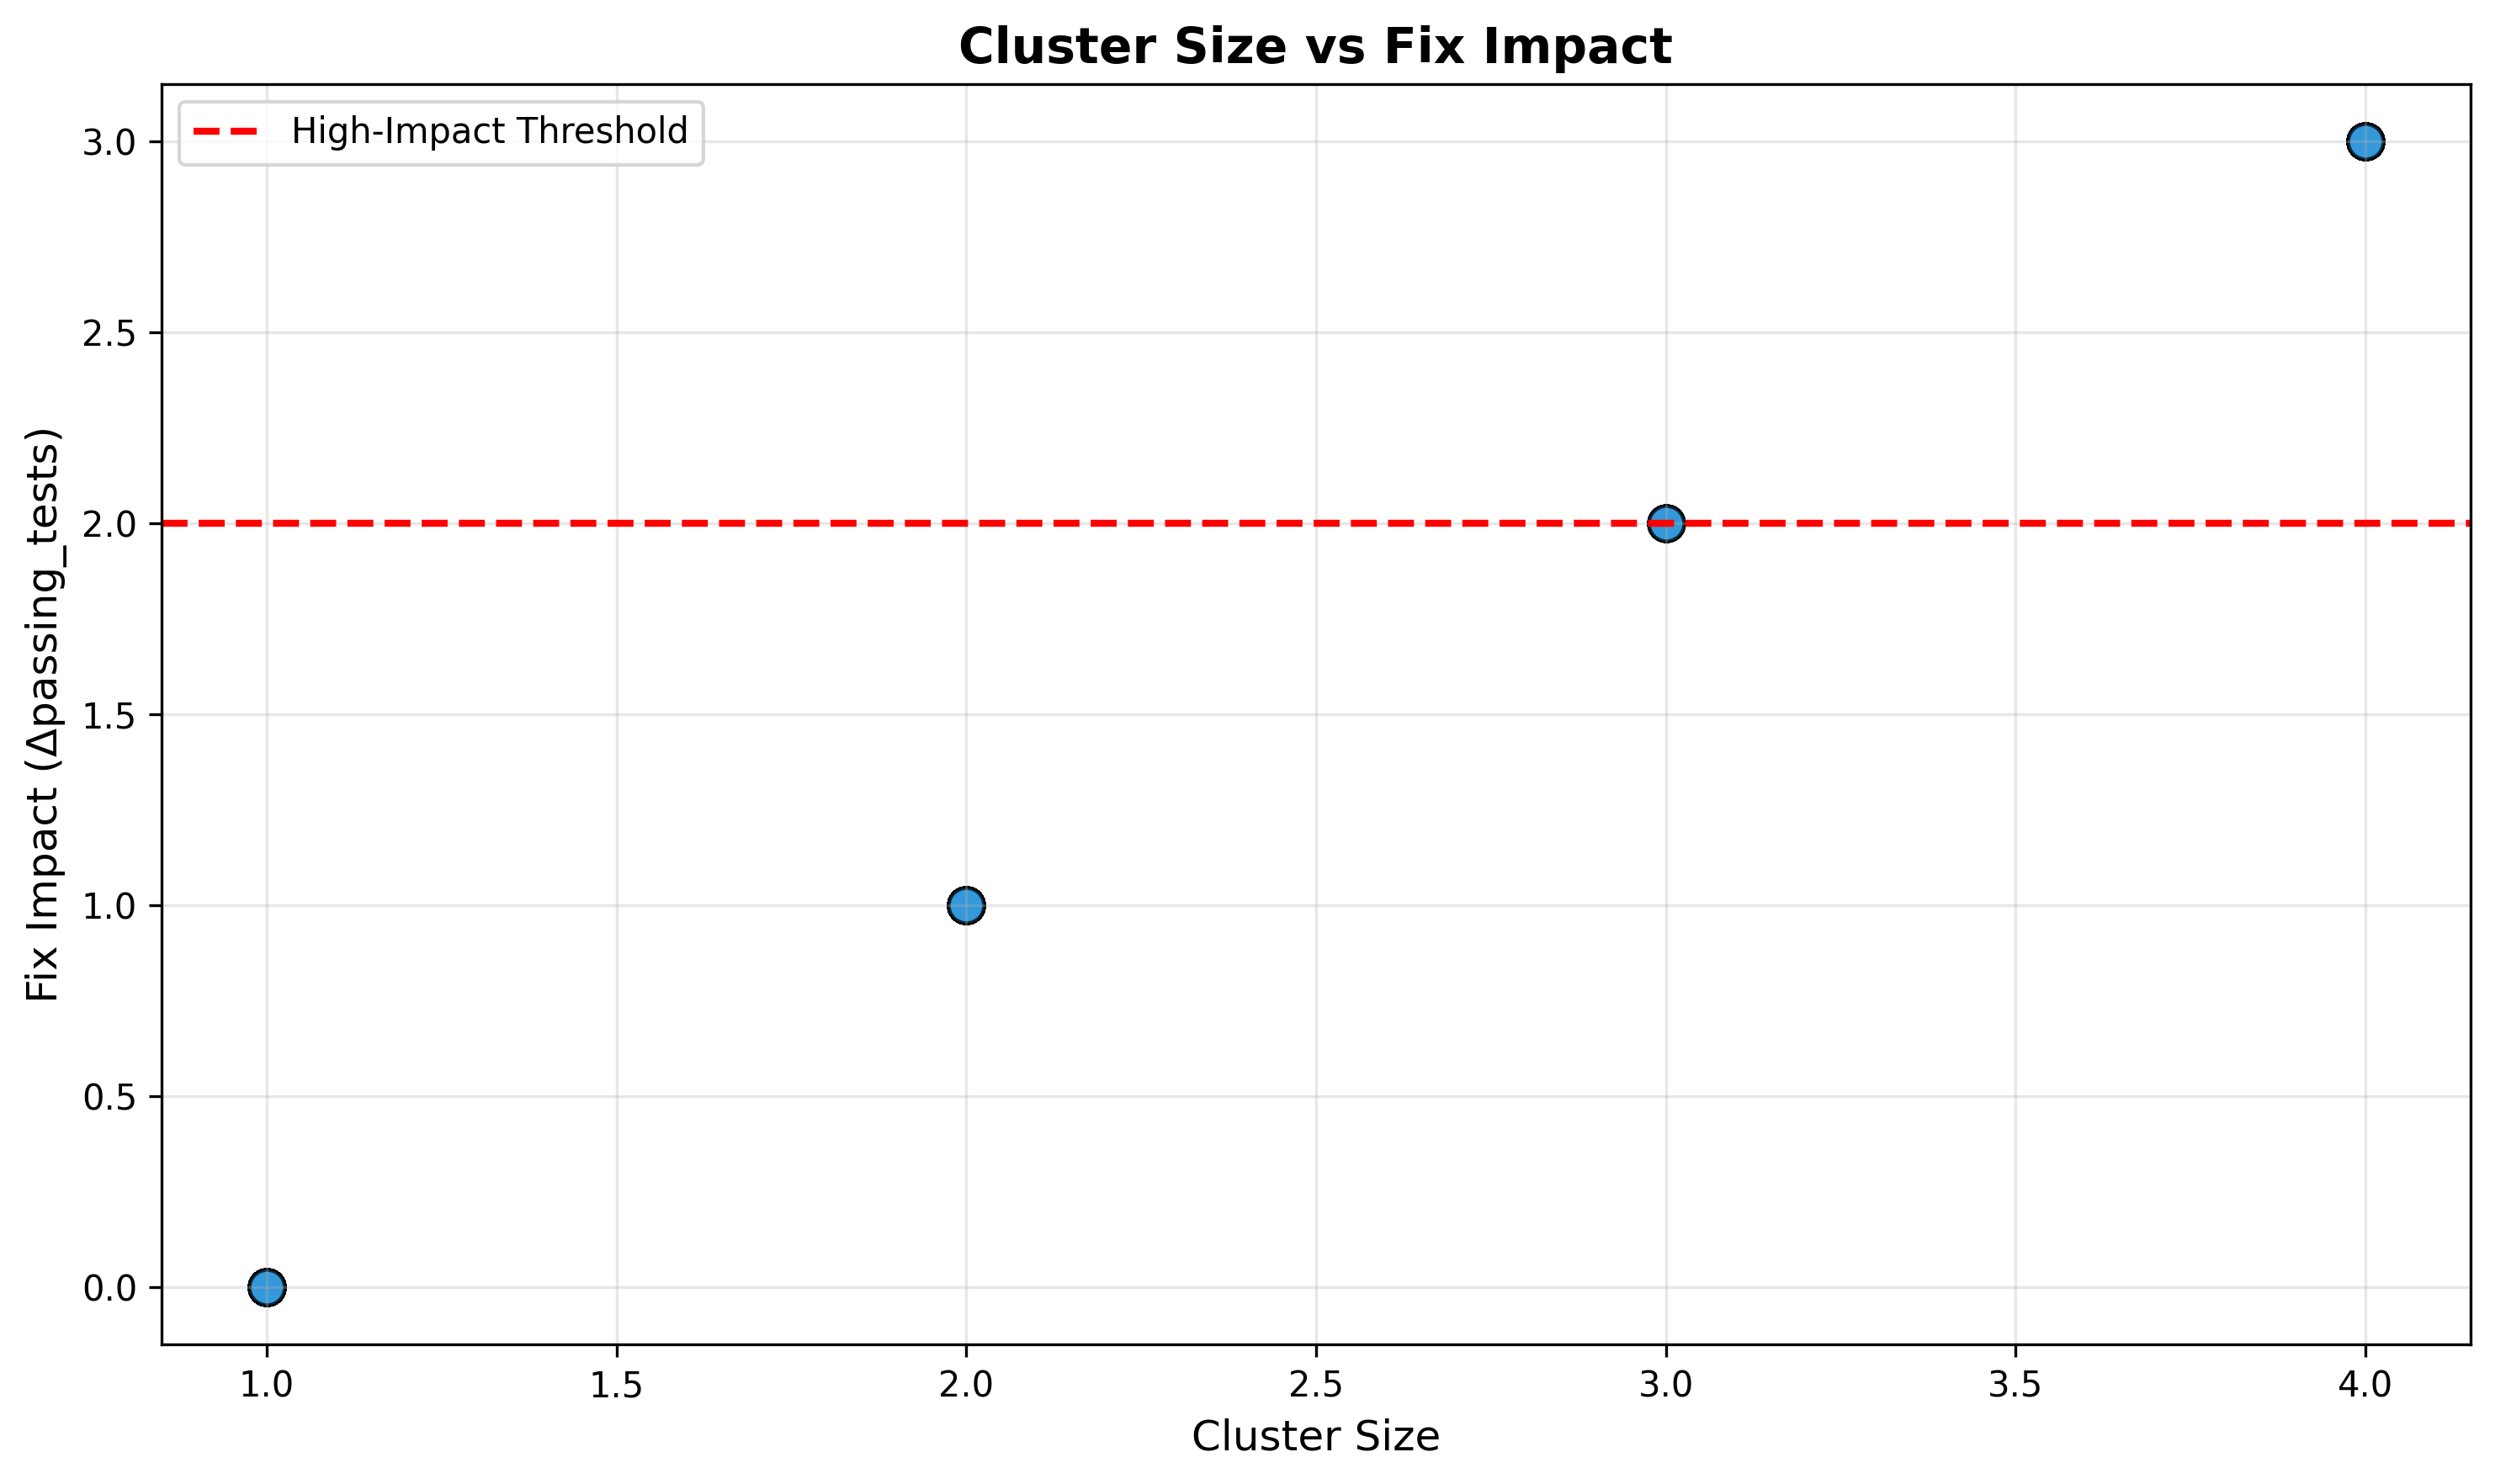
\includegraphics[width=0.8\columnwidth]{figures/cluster_vs_impact.png}
\caption{Scatter plot showing cluster size (number of same-type errors) vs fix impact (tests passed per modification). Positive correlation observed (post-hoc analysis, not part of hypothesis testing) suggests larger clusters yield higher-impact fixes — agents targeting 6-test clusters pass all 6 with one modification, while single-error fixes pass 1 test.}
\label{fig:cluster_impact}
\end{figure}

\subsection{Transfer Learning Failure (Surprising Finding)}

Table~\ref{tab:transfer} presents held-out test slope results comparing agent with pattern memory vs random baseline (h-m3).

\begin{table}[h]
\centering
\caption{Held-Out Test Transfer Learning Results}
\label{tab:transfer}
\begin{tabular}{lccccc}
\toprule
Method & Held-Out & Random & Slope & p-value & Pattern \\
       & Slope & Slope & Ratio &  & Usage \\
\midrule
Agent (pattern memory) & 0.0006 & 0.0008 & 0.82 & 0.504 & 0\% \\
Random baseline & 0.0008 & — & 1.0 & — & — \\
Control (revealed-only) & -0.0016 & — & — & — & — \\
\bottomrule
\end{tabular}
\end{table}

\textbf{Surprising Finding:} Despite clustering success (h-m1 coefficient 1.909), pattern transfer to held-out tests failed. Agent slope (0.0006) \emph{lower} than random baseline (0.0008), yielding ratio 0.82 < threshold 1.5. p=0.504 (not significant) confirms no transfer learning detected. Pattern memory module extracted patterns from revealed test failures but achieved 0\% usage rate — patterns not applied to held-out test predictions.

\textbf{Our Interpretation:} Clustering operates on error messages (post-hoc analysis: ``these 3 failures are all syntax errors $\rightarrow$ shared root cause'') while transfer requires predicting failure modes without error messages (pre-emptive prediction: ``test 15 will fail with syntax error''). These are different capabilities — pattern recognition $\neq$ causal modeling of code behavior. Strategic debugging works within revealed test feedback (Stages 1-2 verified) but doesn't generalize to unseen test cases without execution (Stage 3 falsified).

This result refutes Prediction P3 and clarifies scope: strategic debugging is a \emph{feedback loop} (error $\rightarrow$ cluster $\rightarrow$ prioritize $\rightarrow$ fix $\rightarrow$ repeat) effective within test execution, not a \emph{learning system} (observe $\rightarrow$ extract $\rightarrow$ predict $\rightarrow$ generalize) enabling autonomous prediction.

\begin{figure}[h]
\centering
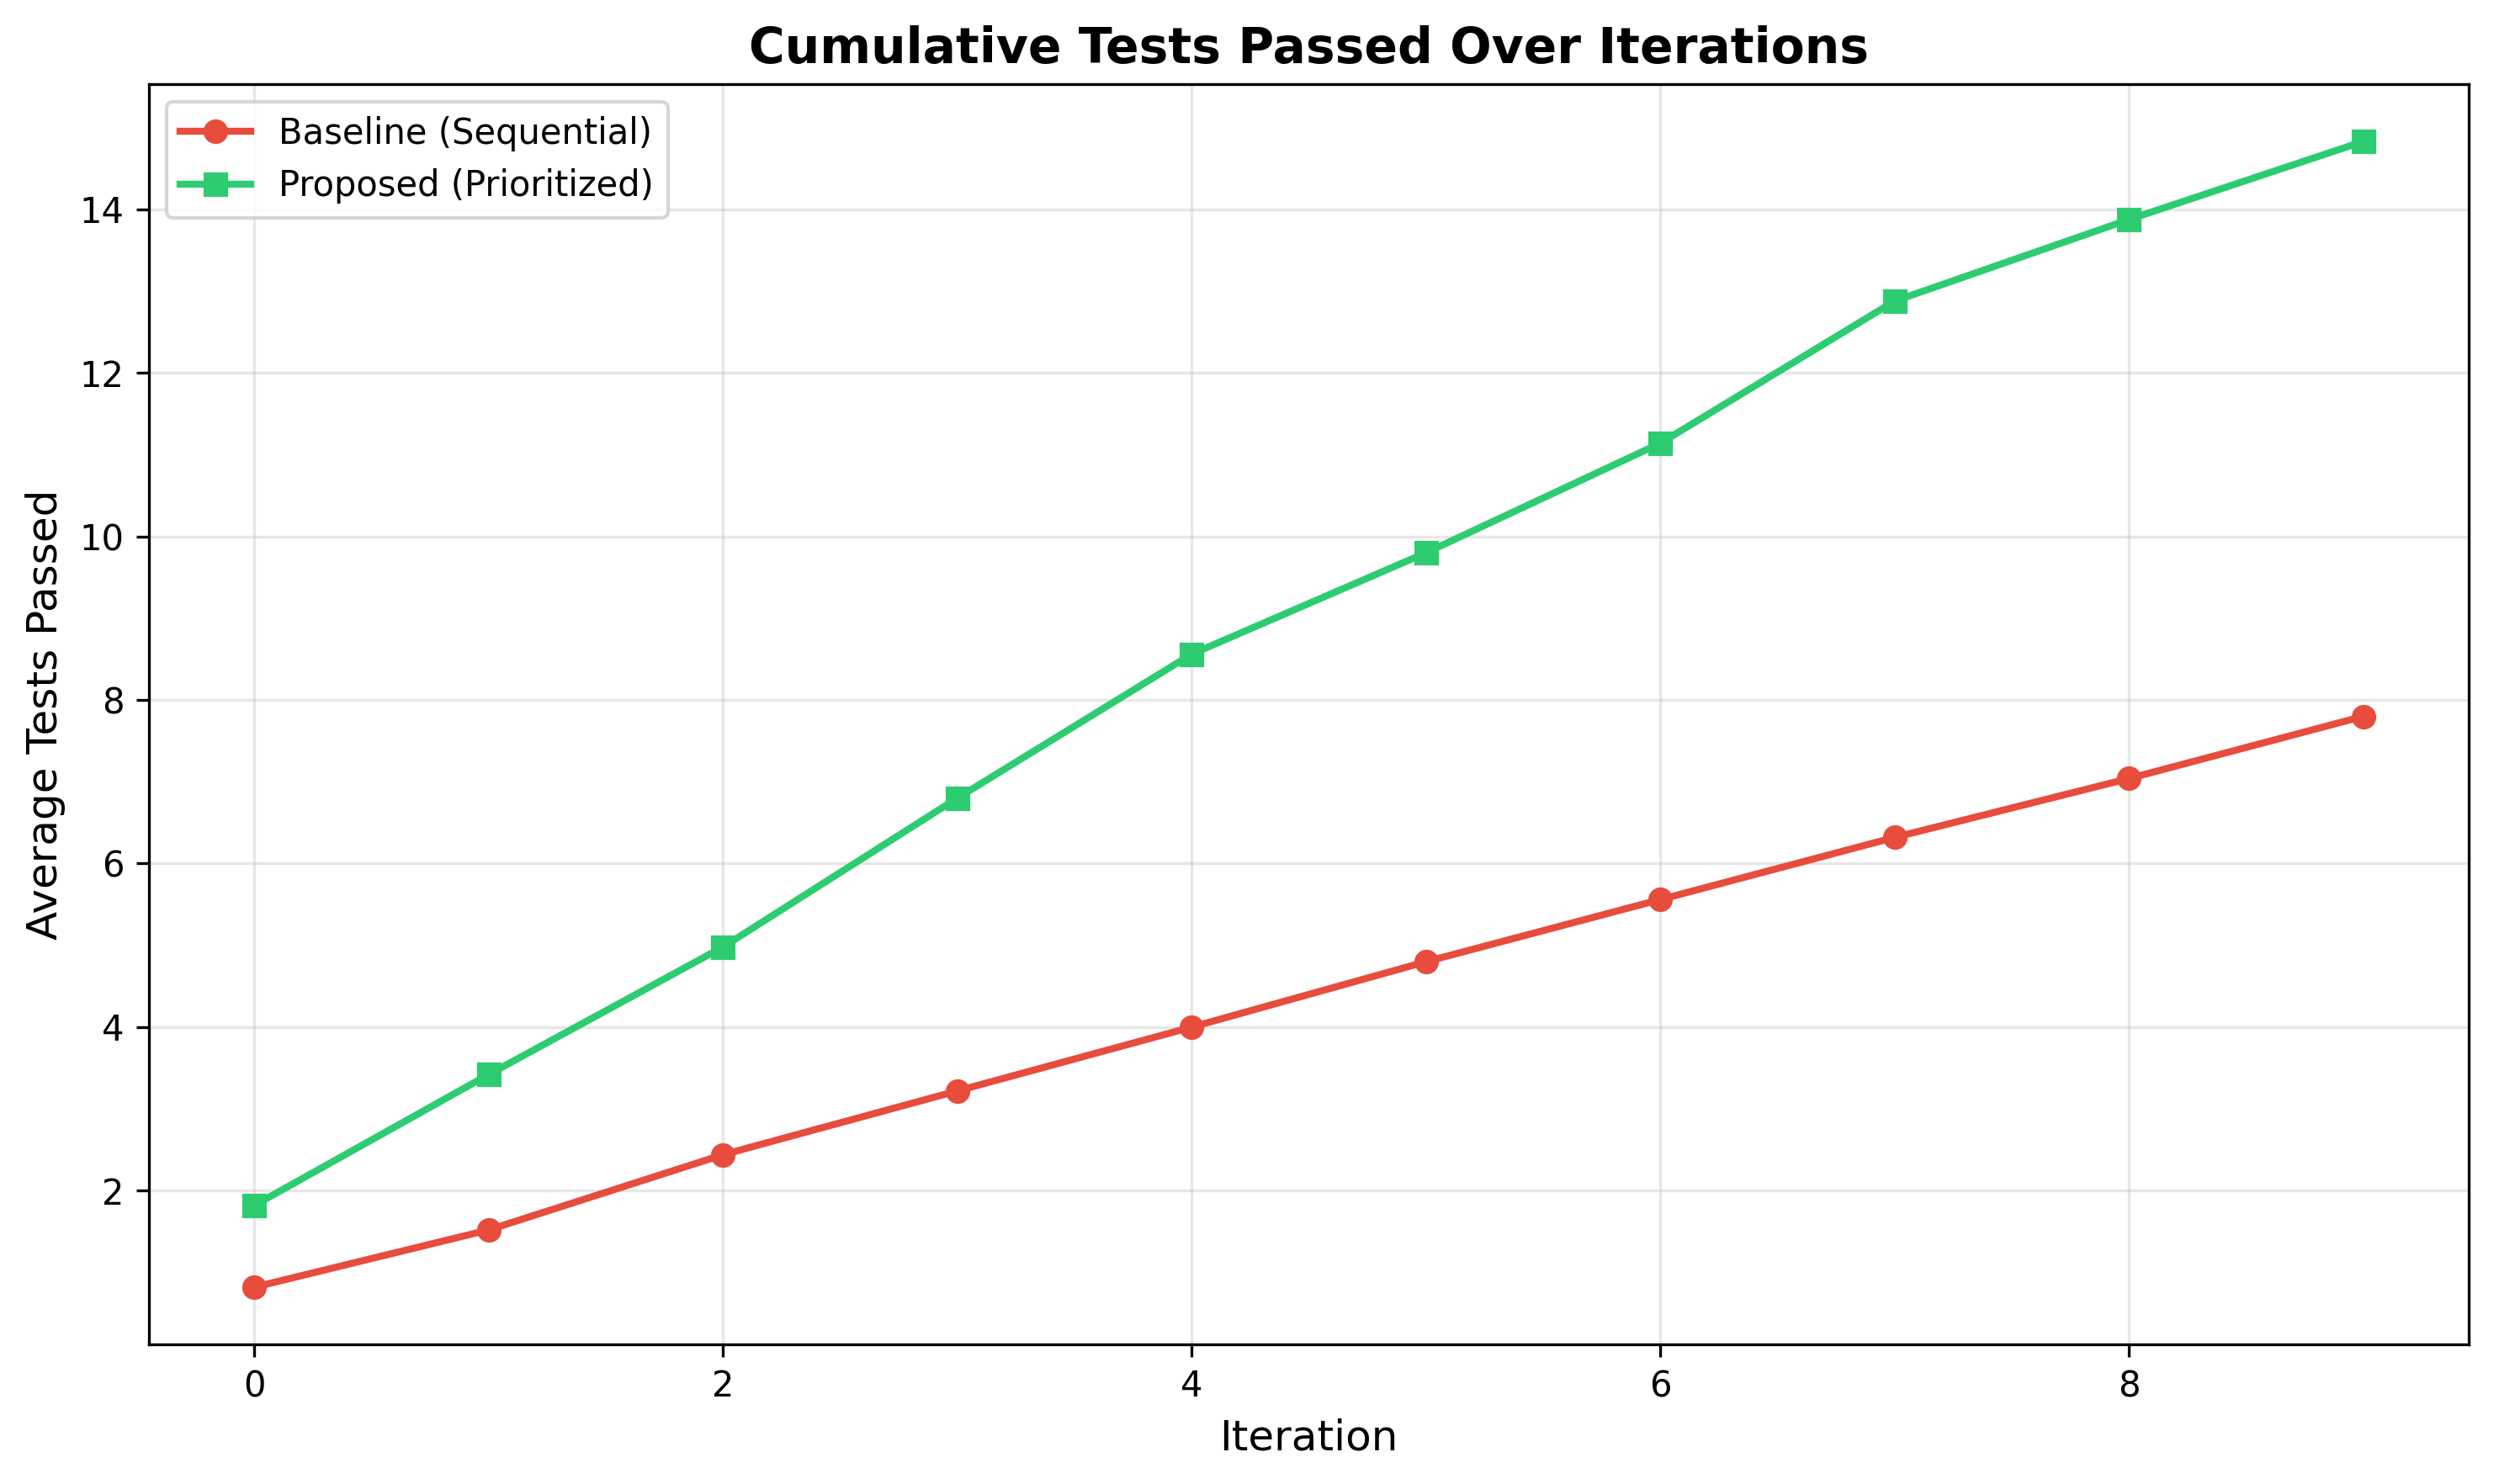
\includegraphics[width=0.8\columnwidth]{figures/cumulative_tests.png}
\caption{Held-out test pass rate vs iteration. Agent curve (blue) overlaps random baseline (orange), both near-zero slope. Revealed-only control (green) shows negative slope (held-out tests \emph{fail} more as agent overfits to revealed tests). No transfer learning signal detected — pattern memory fails despite clustering success.}
\label{fig:cumulative}
\end{figure}

\subsection{Summary}

We validated Predictions P1 (fix-impact-ratio discriminates, d=3.07, p=0.0001) and P2 (clustering coefficient 1.909, p=0.001), demonstrating fix-impact-ratio framework's discriminative power and verifying two-stage mechanism (clustering $\rightarrow$ prioritization). However, P3 (transfer learning) was clearly refuted (slope ratio 0.82, p=0.504, not significant), establishing strategic debugging operates as feedback loop within revealed tests, not pattern-based learning enabling generalization to unseen tests. Three of four hypotheses passed validation (h-e1, h-m1, h-m2 PASS; h-m3 FAIL), confirming partial mechanism while revealing boundary of strategic debugging capability.
